%%%%%%%%%%%%%%%%%%%%%%%%%%%%%%%%%%%%%%%%%%%%%%%%%%%%%%%%%%%%%%%%%%%%%%%%%%%%%%%%
%2345678901234567890123456789012345678901234567890123456789012345678901234567890
%        1         2         3         4         5         6         7         8

\documentclass[12pt, conference]{ieeeconf}

\overrideIEEEmargins
% See the \addtolength command later in the file to balance the column lengths
% on the last page of the document

% Reduce space between figures and text
\setlength{\textfloatsep}{5pt}

\usepackage[utf8]{inputenc}
\usepackage[T1]{fontenc}
\usepackage{float}
\usepackage{graphics}
\usepackage{graphicx}
\usepackage{nth}
\usepackage{pgfplots}
\usepackage{titlesec}
\usepackage[backend=biber,style=ieee]{biblatex}
\usepackage{multirow}
\usepackage{algorithm}
\usepackage{algpseudocode}

\newcommand{\todo}{\colorbox{red}{TODO}}
\newcommand{\todocite}{\colorbox{red}{CITE}}

\addbibresource{references.bib}
\renewcommand*{\bibfont}{\small}

% Defaults
% \setlength{\textfloatsep}{10pt plus 1.0pt minus 2.0pt}
% \setlength{\floatsep}{12pt plus 2.0pt minus 2.0pt}
% \setlength{\intextsep}{12pt plus 2.0pt minus 2.0pt}

% \setlength{\textfloatsep}{0pt plus 1.0pt minus 2.0pt}
\setlength{\floatsep}{3pt plus 2.0pt minus 2.0pt}
\setlength{\intextsep}{3pt plus 2.0pt minus 2.0pt}

\graphicspath{{./figures/}}

\title{\LARGE \bf Practical Analysis of Hybrid Sorting Algorithms}
\author{Joshua Arulsamy}

\author{\parbox{3 in}{
\centering
Joshua Arulsamy\\
University of Wyoming\\
{\tt\small jarulsam@uwyo.edu}}}

\begin{document}

\maketitle
\thispagestyle{plain}
\pagestyle{plain}
\nocite{*}

%%%%%%%%%%%%%%%%%%%%%%%%%%%%%%%%%%%%%%%%%%%%%%%%%%%%%%%%%%%%%%%%%%%%%%%%%%%%%%%%
\begin{abstract}

  Sorting items according to some comparator is a common task in modern
  computing. Most modern applications require data of varying sizes to be sorted
  in a performant manner. Such widespread need for fast, generic, sorting
  functions has resulted in all modern programming languages including a sorting
  function within their respective standard libraries. In the case of the C
  programming language, Quicksort and Mergesort are typically implemented, since
  these algorithms perform very well in the general case. However, combining
  these algorithms with other tertiary sorting algorithms, such as insertion
  sort, can offer sizeable performance gains in real-world scenarios. This
  research investigates the impact sorting algorithm hybridization has on
  performance on a wide variety of system configurations, and proposes a new
  \texttt{qsort} implementation for glibc which outperforms the current
  implementation by upwards of 15\%.

\end{abstract}

%%%%%%%%%%%%%%%%%%%%%%%%%%%%%%%%%%%%%%%%%%%%%%%%%%%%%%%%%%%%%%%%%%%%%%%%%%%%%%%%
\section{INTRODUCTION}

Most applications require data to be arranged in a certain order. The procedure
of reordering data according to some comparator is called sorting. Sorting can
be found in nearly every computer system today. From databases to payment
processing systems, data is constantly being sorted. The near omnipresent need
for performant sorting implementations has resulted in most major programming
languages including a type-generic sorting function within their standard
libraries. These standard implementations can use a variety of algorithms
internally, such as Quicksort, Mergesort, and many others, however, rarely does
a single algorithm perform exceptionally well. Often, these algorithms are
paired with one or more specialized sorting algorithms to offer sizeable
performance benefits. These hybrid algorithms include some tuneable parameters,
such as when to switch from one sorting algorithm to another. While these
hybridized algorithms have varying space and time complexities, their actual
performance in real-world scenarios is rarely formally examined, and the values
for these parameters are often chosen arbitrarily by the developers. This paper
analyzes a wide variety of sorting algorithm implementations across varying
system architectures to determine optimal parameter configurations for hybrid
sorting algorithms. This paper also proposes a new performant standard sorting
implementation for GNU's C standard library leveraging Mergesort, insertion
sort, and sorting networks.

\section{BACKGROUND}

Substantial effort has been spent on the analysis of sorting algorithms.
Typically, two major characteristics are considered when studying sorting
algorithms; space and time complexity. Existing analysis of popular sorting
algorithms, such as Quicksort and Mergesort, place substantial emphasis on their
excellent asymptotic complexity in the average case\parencite{glibc}. However,
asymptotic complexity alone does not describe the practical performance of these
algorithms. While Mergesort may have a better asymptotic time complexity in the
worst case than insertion sort (Table \ref{fig:time_complexity_table}), for
small inputs, insertion sort typically outperforms Mergesort by avoiding the
overhead of recursive calls.

\begin{table}[ht]
	\centering
	\resizebox{\columnwidth}{!}{
		\begin{tabular}{|c|lll|}
			\hline
			\textbf{Algorithm} & \multicolumn{3}{c|}{\textbf{Time Complexity}}                                                                                 \\ \hline
			                   & \multicolumn{1}{l|}{\textbf{Best}}            & \multicolumn{1}{l|}{\textbf{Average}}         & \textbf{Worst}                \\ \hline
			Quicksort          & \multicolumn{1}{l|}{$\Omega(n\log{(n)})$}     & \multicolumn{1}{l|}{$\Theta(n\log{(n)})$}     & $\mathcal{O}(n^{2})$          \\ \hline
			Mergesort          & \multicolumn{1}{l|}{$\Omega(n\log{(n)})$}     & \multicolumn{1}{l|}{$\Theta(n\log{(n)})$}     & $\mathcal{O}(n\log{(n)})$     \\ \hline
			Heapsort           & \multicolumn{1}{l|}{$\Omega(n\log{(n)})$}     & \multicolumn{1}{l|}{$\Theta(n\log{(n)})$}     & $\mathcal{O}(n\log{(n)})$     \\ \hline
			Bubble Sort        & \multicolumn{1}{l|}{$\Omega(n)$}              & \multicolumn{1}{l|}{$\Theta(n^{2})$}          & $\mathcal{O}(n\log{(n)})$     \\ \hline
			Insertion Sort     & \multicolumn{1}{l|}{$\Omega(n)$}              & \multicolumn{1}{l|}{$\Theta(n^{2})$}          & $\mathcal{O}(n^{2})$          \\ \hline
			Tree Sort          & \multicolumn{1}{l|}{$\Omega(n\log{(n)})$}     & \multicolumn{1}{l|}{$\Theta(n\log(n))$}       & $\mathcal{O}(n^{2})$          \\ \hline
			Shell Sort         & \multicolumn{1}{l|}{$\Omega(n\log{(n)})$}     & \multicolumn{1}{l|}{$\Theta(n(\log(n))^{2})$} & $\mathcal{O}(n(\log(n))^{2})$ \\ \hline
		\end{tabular}}
	\caption{Sorting algorithm asymptotic time complexities}
	\label{fig:time_complexity_table}
\end{table}

Most of these algorithms have not been sufficiently benchmarked in real world
scenarios to determine an optimal implementation for common inputs. Evaluating
specific scenarios where an algorithm performs well may lead to better sorting
function implementations by combining several algorithms or excluding algorithms
in specific situations. Since sorting is used so ubiquitously, even incremental
improvements to standard library sorting implementations can broadly influence
the performance of many different applications. Such an analysis does not
presently exist, marking an area in obvious need of further investigation.

\subsection{General Purpose Algorithms}

Of the well known sorting algorithms, several are used for general sorting
tasks, such as Quicksort, Mergesort, Heapsort, and Introsort. Quicksort has been
a staple algorithm for decades. It is well known to be easy to implement and
works well for a variety of input data. Quicksort requires a constant amount of
extra memory independent of the size of the input, making it an obvious choice
in resource constrained environments. However, in the advent of modern computing
where using auxiliary memory to improve performance is much more common,
Quicksort tends to fall behind other algorithms. Quicksort's performance is also
primarily dictated by the selection of a suitable pivot value. Poor pivot
selections can lead to worse performance. Simple implementations usually choose
the left-most value of the input as the pivot, however this offers poor
performance in many circumstances, for example, if the input is reverse sorted.
So most implementations use a slightly more complex and costly pivot selection
process such as \textit{median-of-three}\parencite{Bentley1993EngineeringAS}.

The increased memory availability of modern systems and the difficulty of good
pivot selection within Quicksort has motivated many standard libraries -- such
as GNU's libc -- to default to using Mergesort, falling back to Quicksort only
when memory requirements are too high\parencite{glibc}. Such implementations are
typically more performant in most cases, since Mergesort can leverage extra
memory for better performance, and maintain usability even in memory constrained
environments.

\subsection{Specialized Algorithms}

A few algorithms used in specialized circumstances are also evaluated, most
notably, various sorting network implementations, insertion sort, and shell
sort. These algorithms are often regarded as the best sorting algorithms for
extremely small inputs. Since their asymptotic complexity is substantially worse
than a general purpose sorting algorithm their runtime typically grows
exponentially as the input size increases (Table
\ref{fig:time_complexity_table}). However, for small inputs, these algorithms
are highly performant since they avoid the overhead of more complicated
algorithms.

Sorting networks, also commonly referred to as comparator networks, are designed
to sort fixed numbers of items. Unlike other sorting algorithms, networks cannot
handle arbitrarily large inputs. However, even with this constraint, sorting
networks are still commonly used. They are highly performant in instances where
the input is extremely small. Since the order at which elements are compared is
always constant, carefully designing an optimal sorting network which minimizes
the number of comparisons will likely benefit from modern CPU branch
predictions. For small input sizes ($n < 16$), minimal comparison optimal
sorting networks have been thoroughly investigated, and their performance is
proven\parencite{knuth_networks}\parencite{engineering_fast_sorters}. For
slightly larger inputs, insertion sort is a prime candidate. Unlike Mergesort
and Quicksort, insertion sort is simple. The minimal overhead typically allows
insertion sort to outperform more complicated algorithms for small inputs. These
algorithms are prime candidates for hybridization with general purpose
algorithms.


\section{Proposed Algorithm}

General purpose sorting algorithms are typically difficult to optimize
uniformly. Since these implementations very often live in standard libraries,
use-case specific optimizations are not feasible. During runtime, quick,
low-overhead analysis about the input can reveal opportunities for
input-specific optimizations. More esoteric sorting methods, such as TimSort,
take advantage of such analysis during sorting to improve performance in most
real-world cases. However, for small input sizes, the overhead from such an
analysis often contributes more to the overall runtime, than even utilizing an
algorithm ill-suited for that specific input\parencite{the_basic_algorithms}.
This motivates placing significant importance on the size of the input itself.

Comparing the input size against predefined threshold values is cheap and can
help pick an algorithm. Since such comparisons are so cheap, they can be
repeated during recursive calls of other algorithms. The proposed algorithm is
an optimized version of Mergesort (Algorithm \ref{alg:merge_sort}) which checks
the size of each subarray during each recursive call. If the subarray's length
is less than a threshold value, insertion sort (Algorithm
\ref{alg:insertion_sort}) is used instead. In instances where a subarray
contains less than 5 elements, a comparison-optimal network sorting algorithm
(Algorithm \ref{alg:network_sort}) is used instead of insertion sort. Utilizing
secondary algorithms limits the depth of recursive calls substantially.
Practically, this offers significant performance gains, even though there are
additional size comparisons during each recursive
call\parencite{the_basic_algorithms}.

\begin{algorithm}[H]
	\caption{Network Sort}
	\label{alg:network_sort}
	\begin{algorithmic}
		\Procedure{SORT2}{$x$, $y$}
		\State $minPtr \gets \Call{min}{x, y}$
		\If {$x = minPtr$}
		\State $maxPtr \gets y$
		\Else
		\State $maxPtr \gets x$
		\EndIf
		\State $t \gets minPtr$
		\State $y \gets maxPtr$
		\State $x \gets t$
		\EndProcedure

		\Procedure{SORT3}{$a$}
		\State \Call{SORT2}{$a[0]$, $a[2]$}
		\State \Call{SORT2}{$a[0]$, $a[1]$}
		\State \Call{SORT2}{$a[1]$, $a[2]$}
		\EndProcedure

		\Procedure{SORT4}{$a$}
		\State \Call{SORT2}{$a[0]$, $a[2]$}
		\State \Call{SORT2}{$a[1]$, $a[3]$}
		\State \Call{SORT2}{$a[0]$, $a[1]$}
		\State \Call{SORT2}{$a[2]$, $a[3]$}
		\State \Call{SORT2}{$a[1]$, $a[2]$}
		\EndProcedure
	\end{algorithmic}
\end{algorithm}

\begin{algorithm}[H]
	\caption{Insertion Sort}
	\label{alg:insertion_sort}
	\begin{algorithmic}
		\Procedure{INS\_SORT}{a, n}
		\For {$i \gets 1$ to $n$}
		\State $c \gets 1$
		\State $j \gets i - 1$
		\If {$a[j] > a[i]$}
		\State $tmp \gets a[i]$
		\Repeat
		\State $a[j + 1] \gets a[j]$
		\If {$j = 0$}
		\State $c \gets 0$
		\State \textbf{break}
		\EndIf
		\State $j \gets j - 1$
		\Until $a[j] \le tmp$
		\State $a[j + c] \gets tmp$
		\EndIf
		\EndFor
		\EndProcedure
	\end{algorithmic}
\end{algorithm}

\begin{algorithm}[H]
	\caption{Hybridized Merge Sort}
	\label{alg:merge_sort}
	\begin{algorithmic}
		\Procedure{msort}{$a$, $n$, $threshold$}
		\If {$n \le 1$}
		\State \Return
		\EndIf

		\If {$n < threshold$}
		\If {$n = 2$}
		\State \Call{sort2}{$a$, $n$}
		\State \Return
		\ElsIf {$n = 3$}
		\State \Call{sort3}{$a$, $n$}
		\State \Return
		\ElsIf {$n = 4$}
		\State \Call{sort4}{$a$, $n$}
		\State \Return
		\EndIf

		\State \Call{ins\_sort}{$a$, $n$}
		\State \Return
		\EndIf

		\State $n_{1} \gets \frac{n}{2}$
		\State $n_{2} \gets n - n_{1}$
		\State $b_{1} \gets a$
		\State $b_{2} \gets \&b[n_{1}]$

		% Recursively sort two halves.
		\State \Call{msort}{$b_{1}$, $n_{1}$, $threshold$}
		\State \Call{msort}{$b_{2}$, $n_{2}$, $threshold$}

		% Merge the two halves.
		\While {$n_{1} > 0$ and $n_{2} > 0$}
		\If {$b_{1}[0] \le b_{2}[0]$}
		\State $tmp \gets b_{1}$
		\State $b_{1} \gets \&b_{1}[1]$
		\State $n_{1} \gets n_{1} - 1$
		\Else
		\State $tmp \gets b_{2}$
		\State $b_{2} \gets \&b_{2}[1]$
		\State $n_{2} \gets n_{2} - 1$
		\EndIf
		\EndWhile

		\If {$n_{1} > 0$}
		\State copy($tmp$, $b_{1}$, $n_{1}$)
		\EndIf
		\State copy($a$, $tmp$, $n - n_{2}$)
		\EndProcedure
	\end{algorithmic}
\end{algorithm}

\subsection{Implementation}

The actual implementation of the proposed algorithms differ slightly from the
psuedocode descriptions (Algorithm \ref{alg:network_sort},
\ref{alg:insertion_sort}, \& \ref{alg:merge_sort}). Since this investigation is
focused on improving standard library implementations, specifically GNU libc's
\verb|qsort()|, all of these algorithms are implemented in C in a type-generic
fashion in accordance with ISO C standard\parencite{iso_c}. This presents
another opportunity for optimization. Type-generic functions in C are
implemented using \verb|void| pointers -- essentially subverting the type system
itself. Such implementations must take care in maintaining alignment when moving
any elements within a contiguous block of un-typed memory. The catch-all method
for safely manipulating un-typed memory is resorting to \verb|memcpy| and its
family of system calls. However, system calls are extremely expensive and
repeated usage of \verb|memcpy| has a significant performance penalty. This
implementation avoids repeated system calls. Upon invocation, several
preliminary heuristics are immediately examined; size of each element within the
input, total input length, and alignment.

The size of each element and total length of input are used to calculate the
total required auxiliary temporary space for Mergesort. If the required memory
is sufficiently small, it is stack allocated, otherwise it is heap allocated. If
at any time a request for memory fails, Mergesort is abandoned and Quicksort is
utilized. Using some clever pointer arithmetic, the alignment of the input data
is matched against several pre-defined alignments. Depending on the alignment,
the input data can be treated as a known primitive, such as an 32-bit unsigned
integer, making swaps of type-generic inputs essentially cost the same as
swapping primitive integers. In practice, this offers a very sizeable
performance gain. If the size of each individual element is large, indirect
sorting is utilized. A new array is populated with pointers to the original
inputs and the pointers are ordered according to the comparator function. Once
the pointers are correctly ordered, the elements in the original array are
copied to the correct location based on the position of their corresponding
indirect sorting pointer. This way, swaps stay cheap, since the amount of total
memory being moved remains less than 8 bytes per element per swap.


\section{EXPERIMENTAL SETUP}

A small subset of algorithms were chosen for evaluation. Primarily, algorithms
utilized within standard library implementations are of particular interest,
since they are typically highly performant in the general case. Other
complementary algorithms which perform exceptionally well in specific scenarios
were also evaluated. Since this analysis is focused on analyzing and improving
existing implementations, general purpose sorting function were taken from
various standard libraries, such as GNU's libc\parencite{glibc} and musl
libc\parencite{musl_libc}. It is a priority to maintain the applicability of any
optimizations discovered as a result of this evaluation to existing standard
libraries, so any non-comparison based sorting algorithm, such as Radix sort or
Bucket sort, were excluded. Other hybridization combinations were also included,
such as combining Mergesort with just insertion sort, to serve as a comparison.
To evaluate the algorithms, each is timed while sorting the same data $1,000$
times. Finally the mean is calculated for each algorithm. This is done to
minimize noise (time inaccuracy, other processes on the test system, etc.)
during data collection. To illustrate the relationship between the threshold at
which hybridized methods switch algorithms, various threshold values are tested
against the same input data. Several input data sequences were chosen to
represent real-world sorting scenarios, such as already sorted (ascending),
reverse sorted (descending), a repeated single number, pipe organ (ex. 1, 2, 3,
4, 3, 2, 1) and entirely random.

\section{RESULTS}

The proposed algorithm outperforms the existing implementation of \verb|qsort()|
in most circumstances. The threshold value does affect the runtime of these
algorithms substantially, typically offering best performance around 3 to 12.
When picking a suitable threshold value, it is important to consider how the
algorithm will perform in the general case. Based on Fig. \ref{ascending} it may
look appealing to choose a threshold value above 12, since already sorted data
benefits the most from repeated use of low-overhead algorithms (such as
insertion-sort). However, for reverse sorted data, threshold values above 6 have
nearly no performance gain over the existing implementation.

\todo

\begin{figure}[H]
	\centering
	\makebox[\columnwidth]{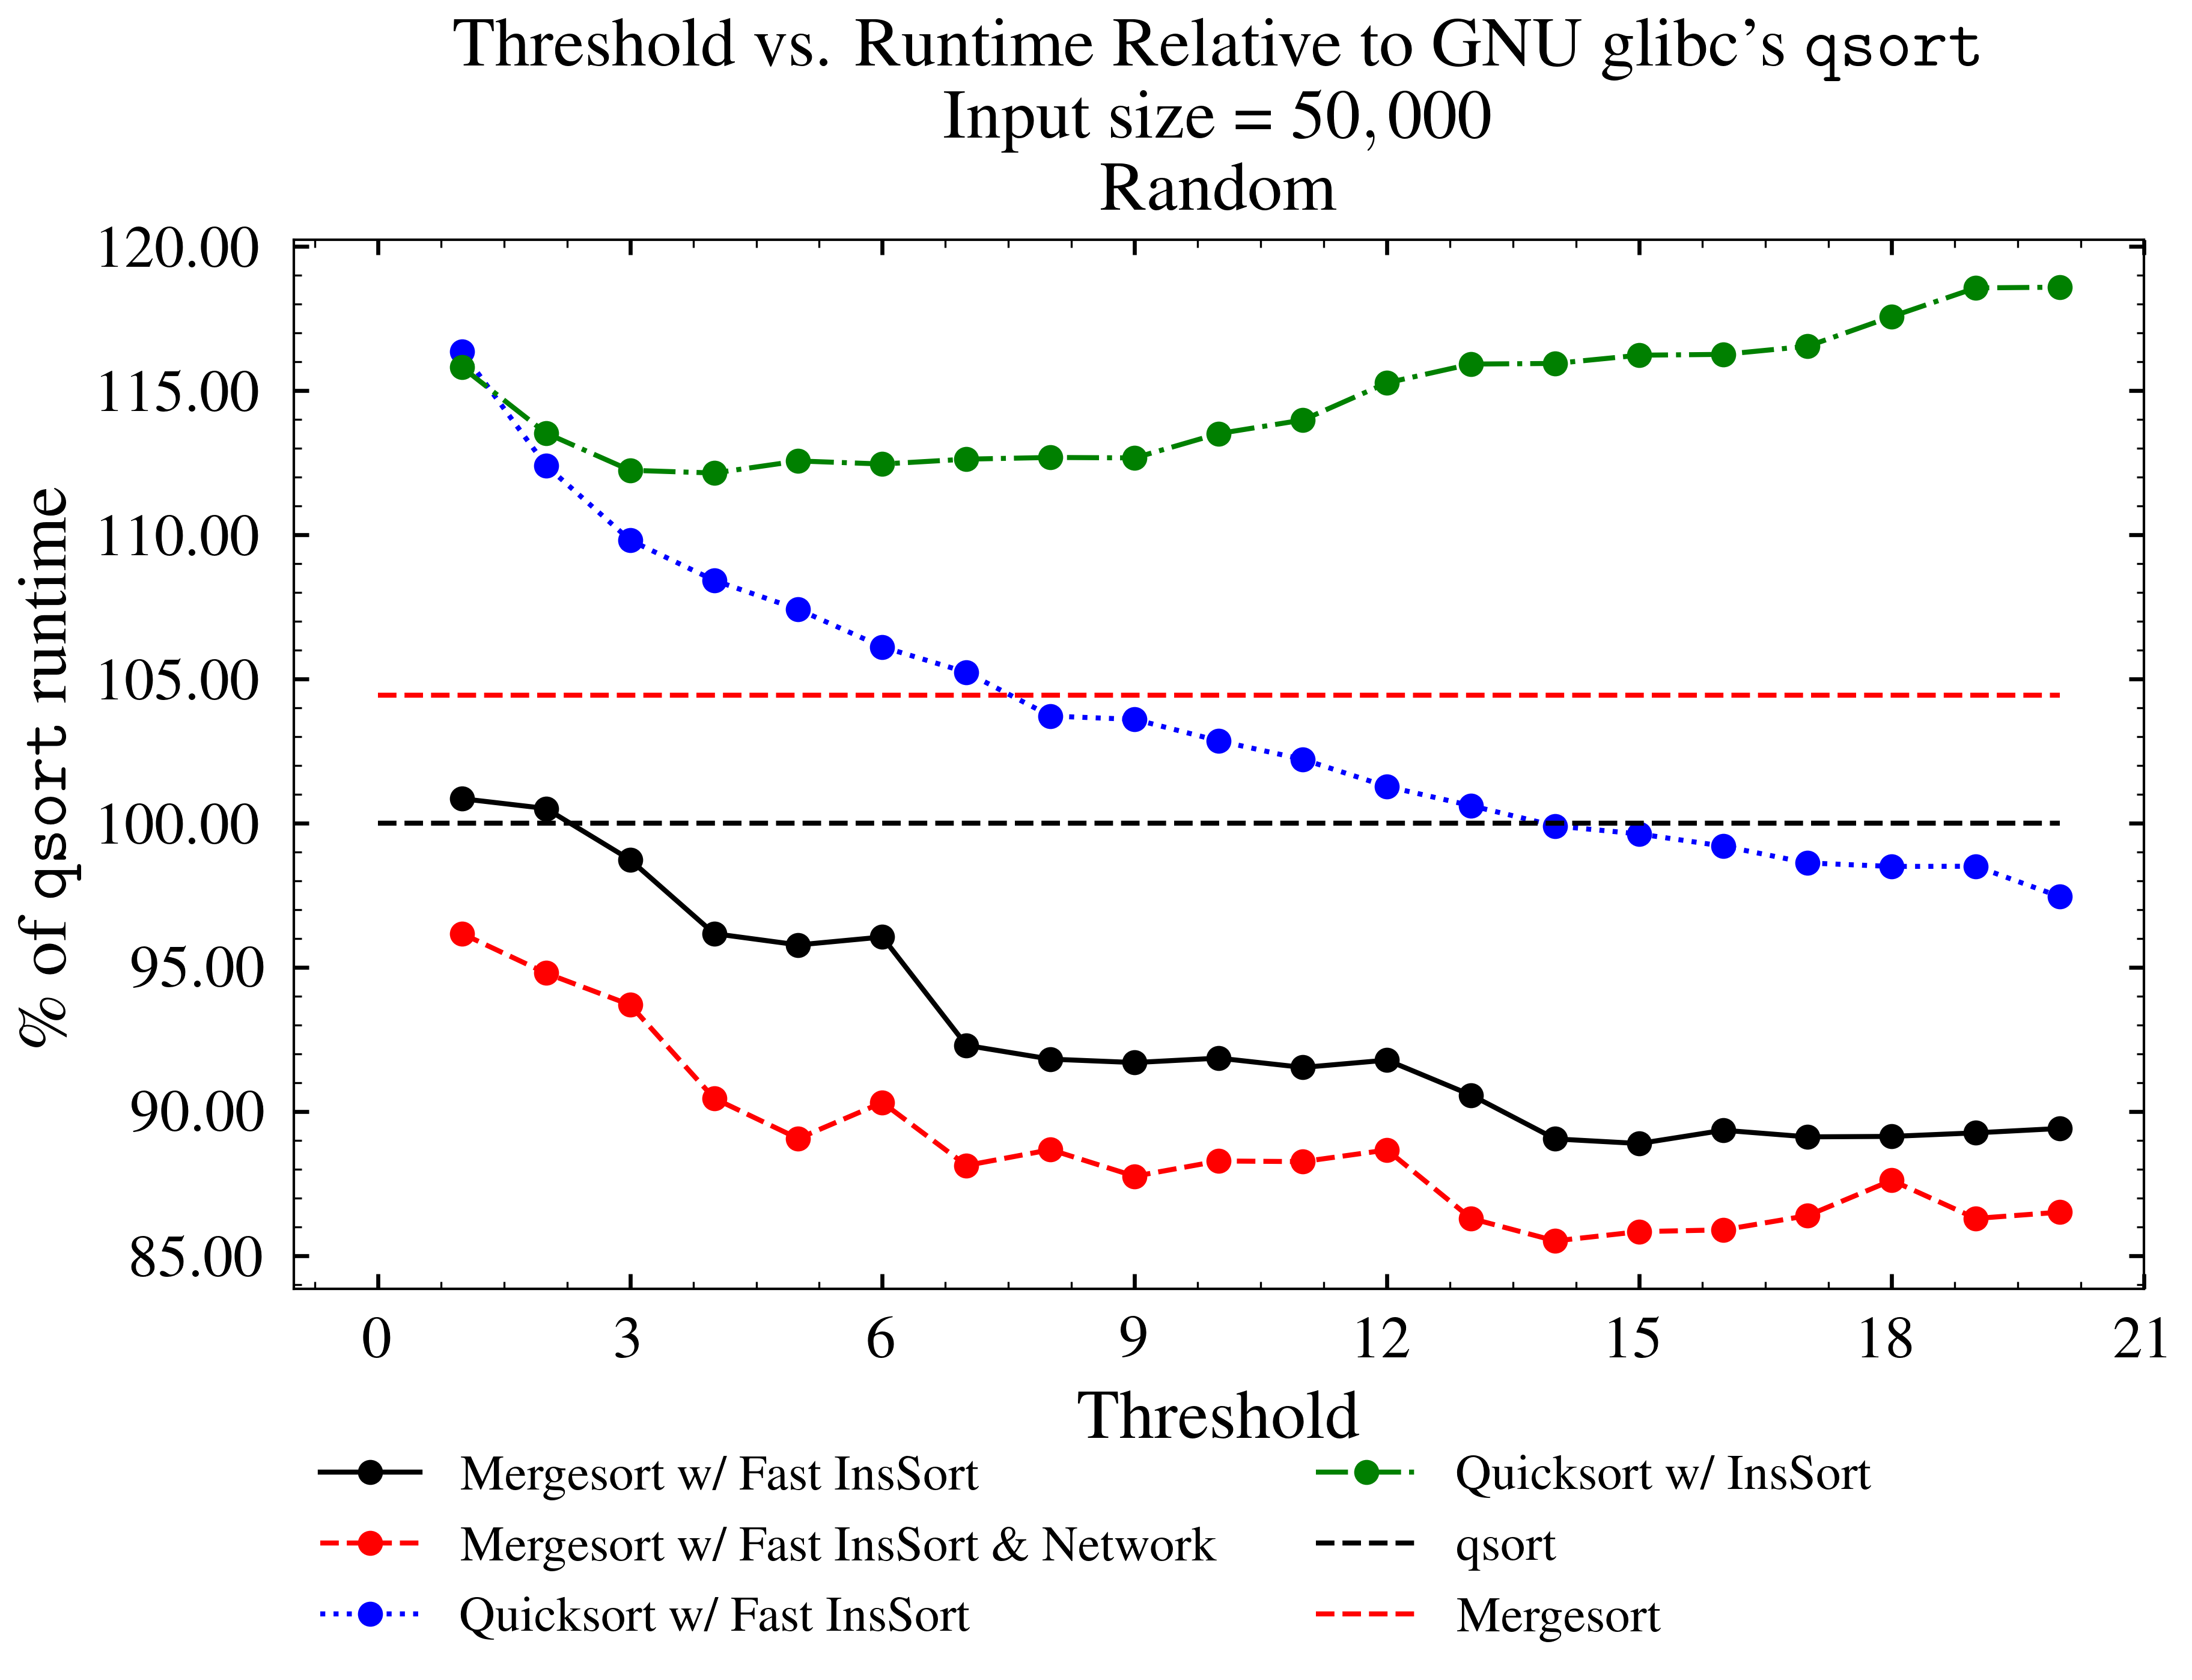
\includegraphics[width=\columnwidth]{random}}
	\caption{Random}
	\label{fig:random}
\end{figure}
\begin{figure}[H]
	\centering
	\makebox[\columnwidth]{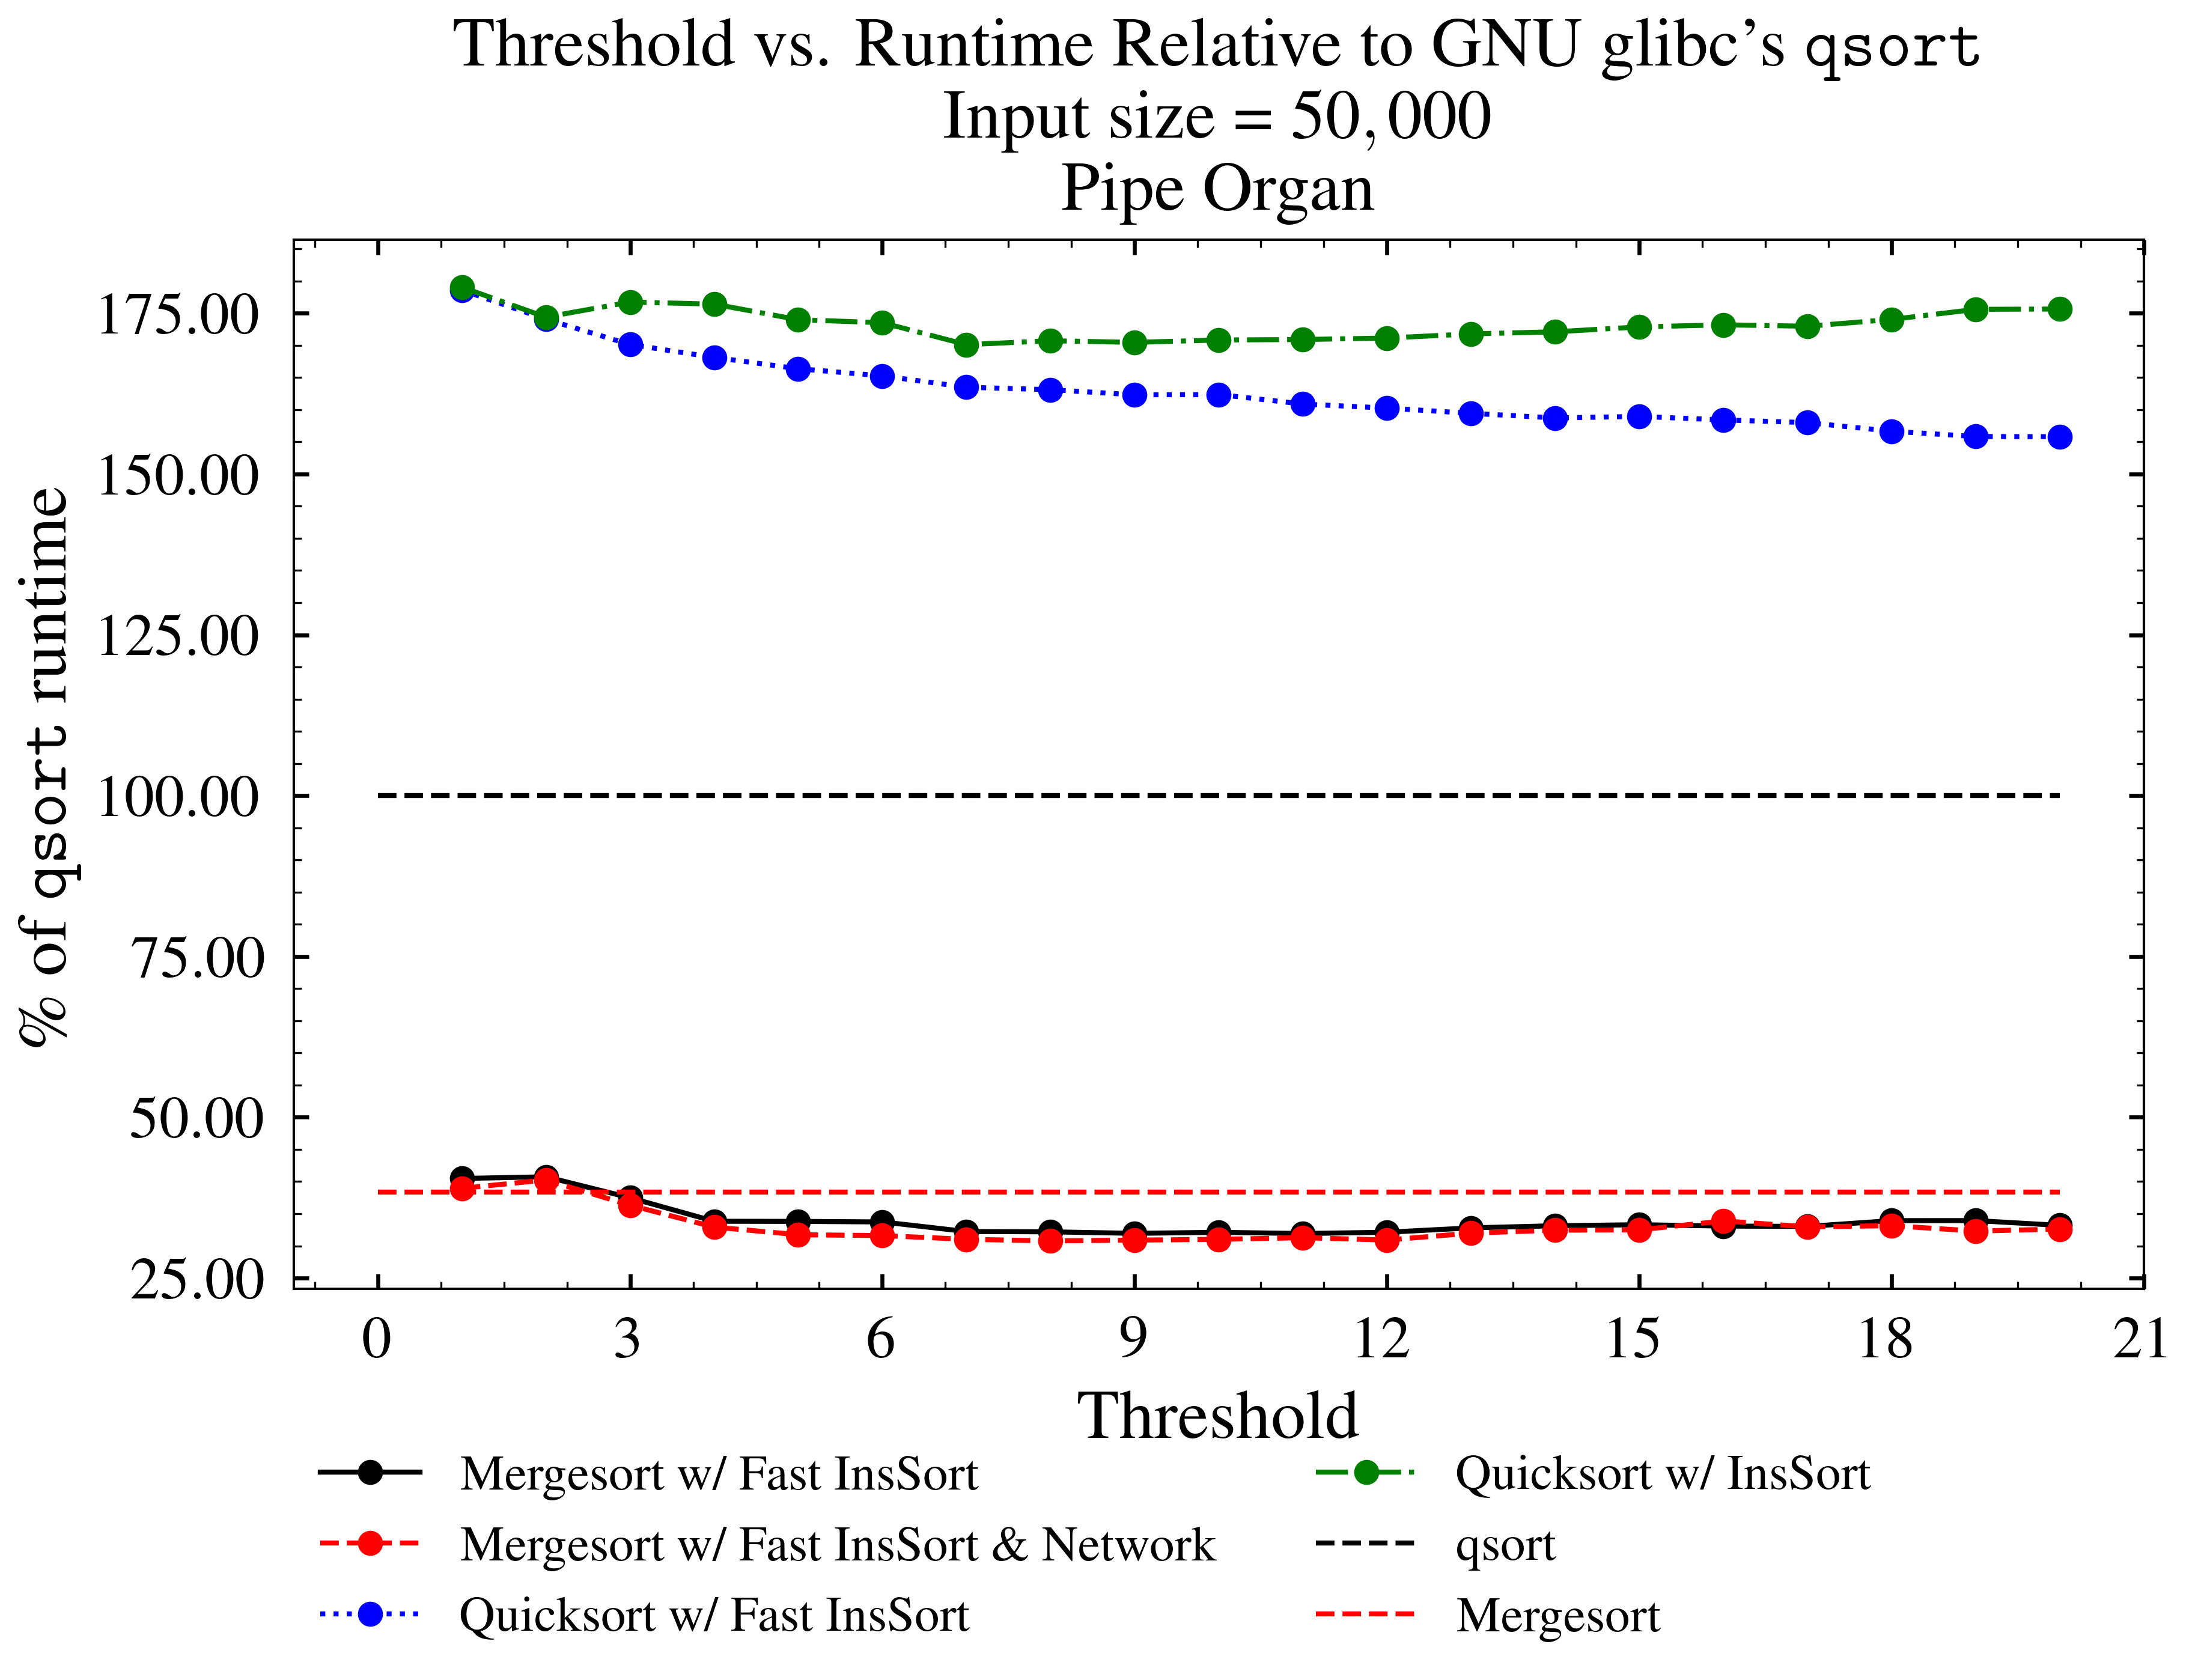
\includegraphics[width=\columnwidth]{pipe_organ}}
	\caption{Pipe Organ}
	\label{fig:pipe_organ}
\end{figure}
\begin{figure}[H]
	\centering
	\makebox[\columnwidth]{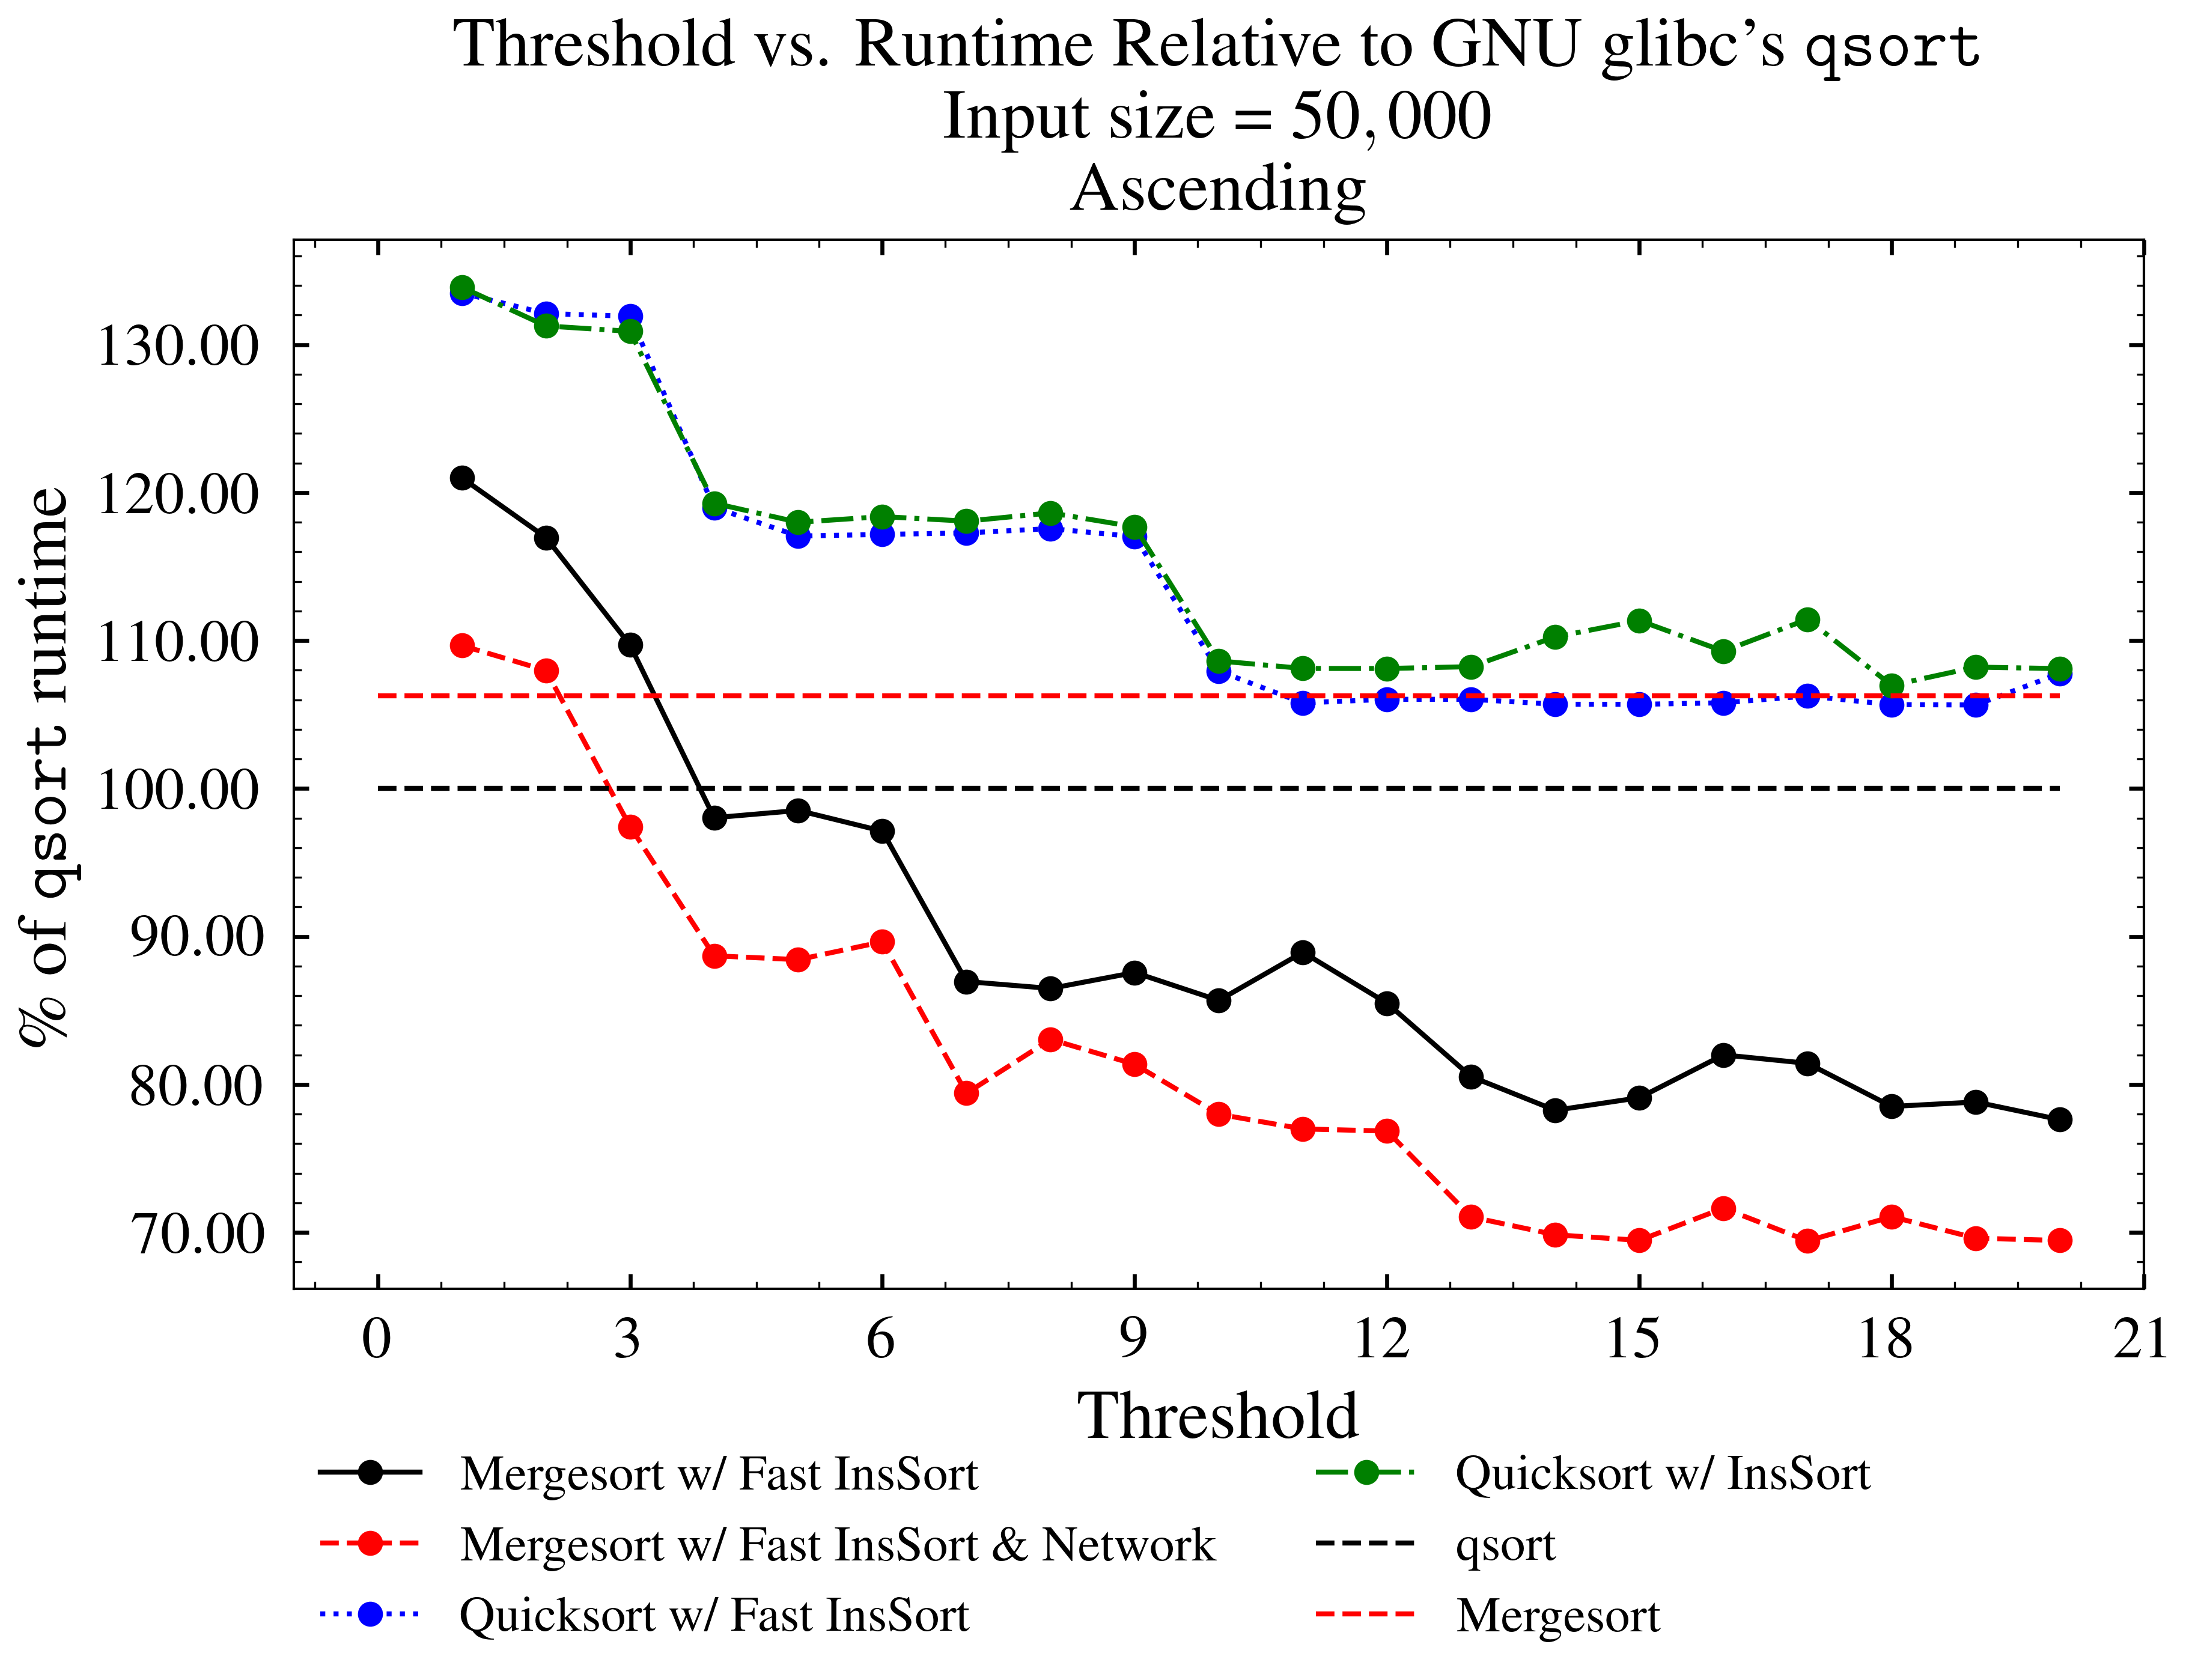
\includegraphics[width=\columnwidth]{ascending}}
	\caption{Ascending}
	\label{fig:ascending}
\end{figure}
\begin{figure}[H]
	\centering
	\makebox[\columnwidth]{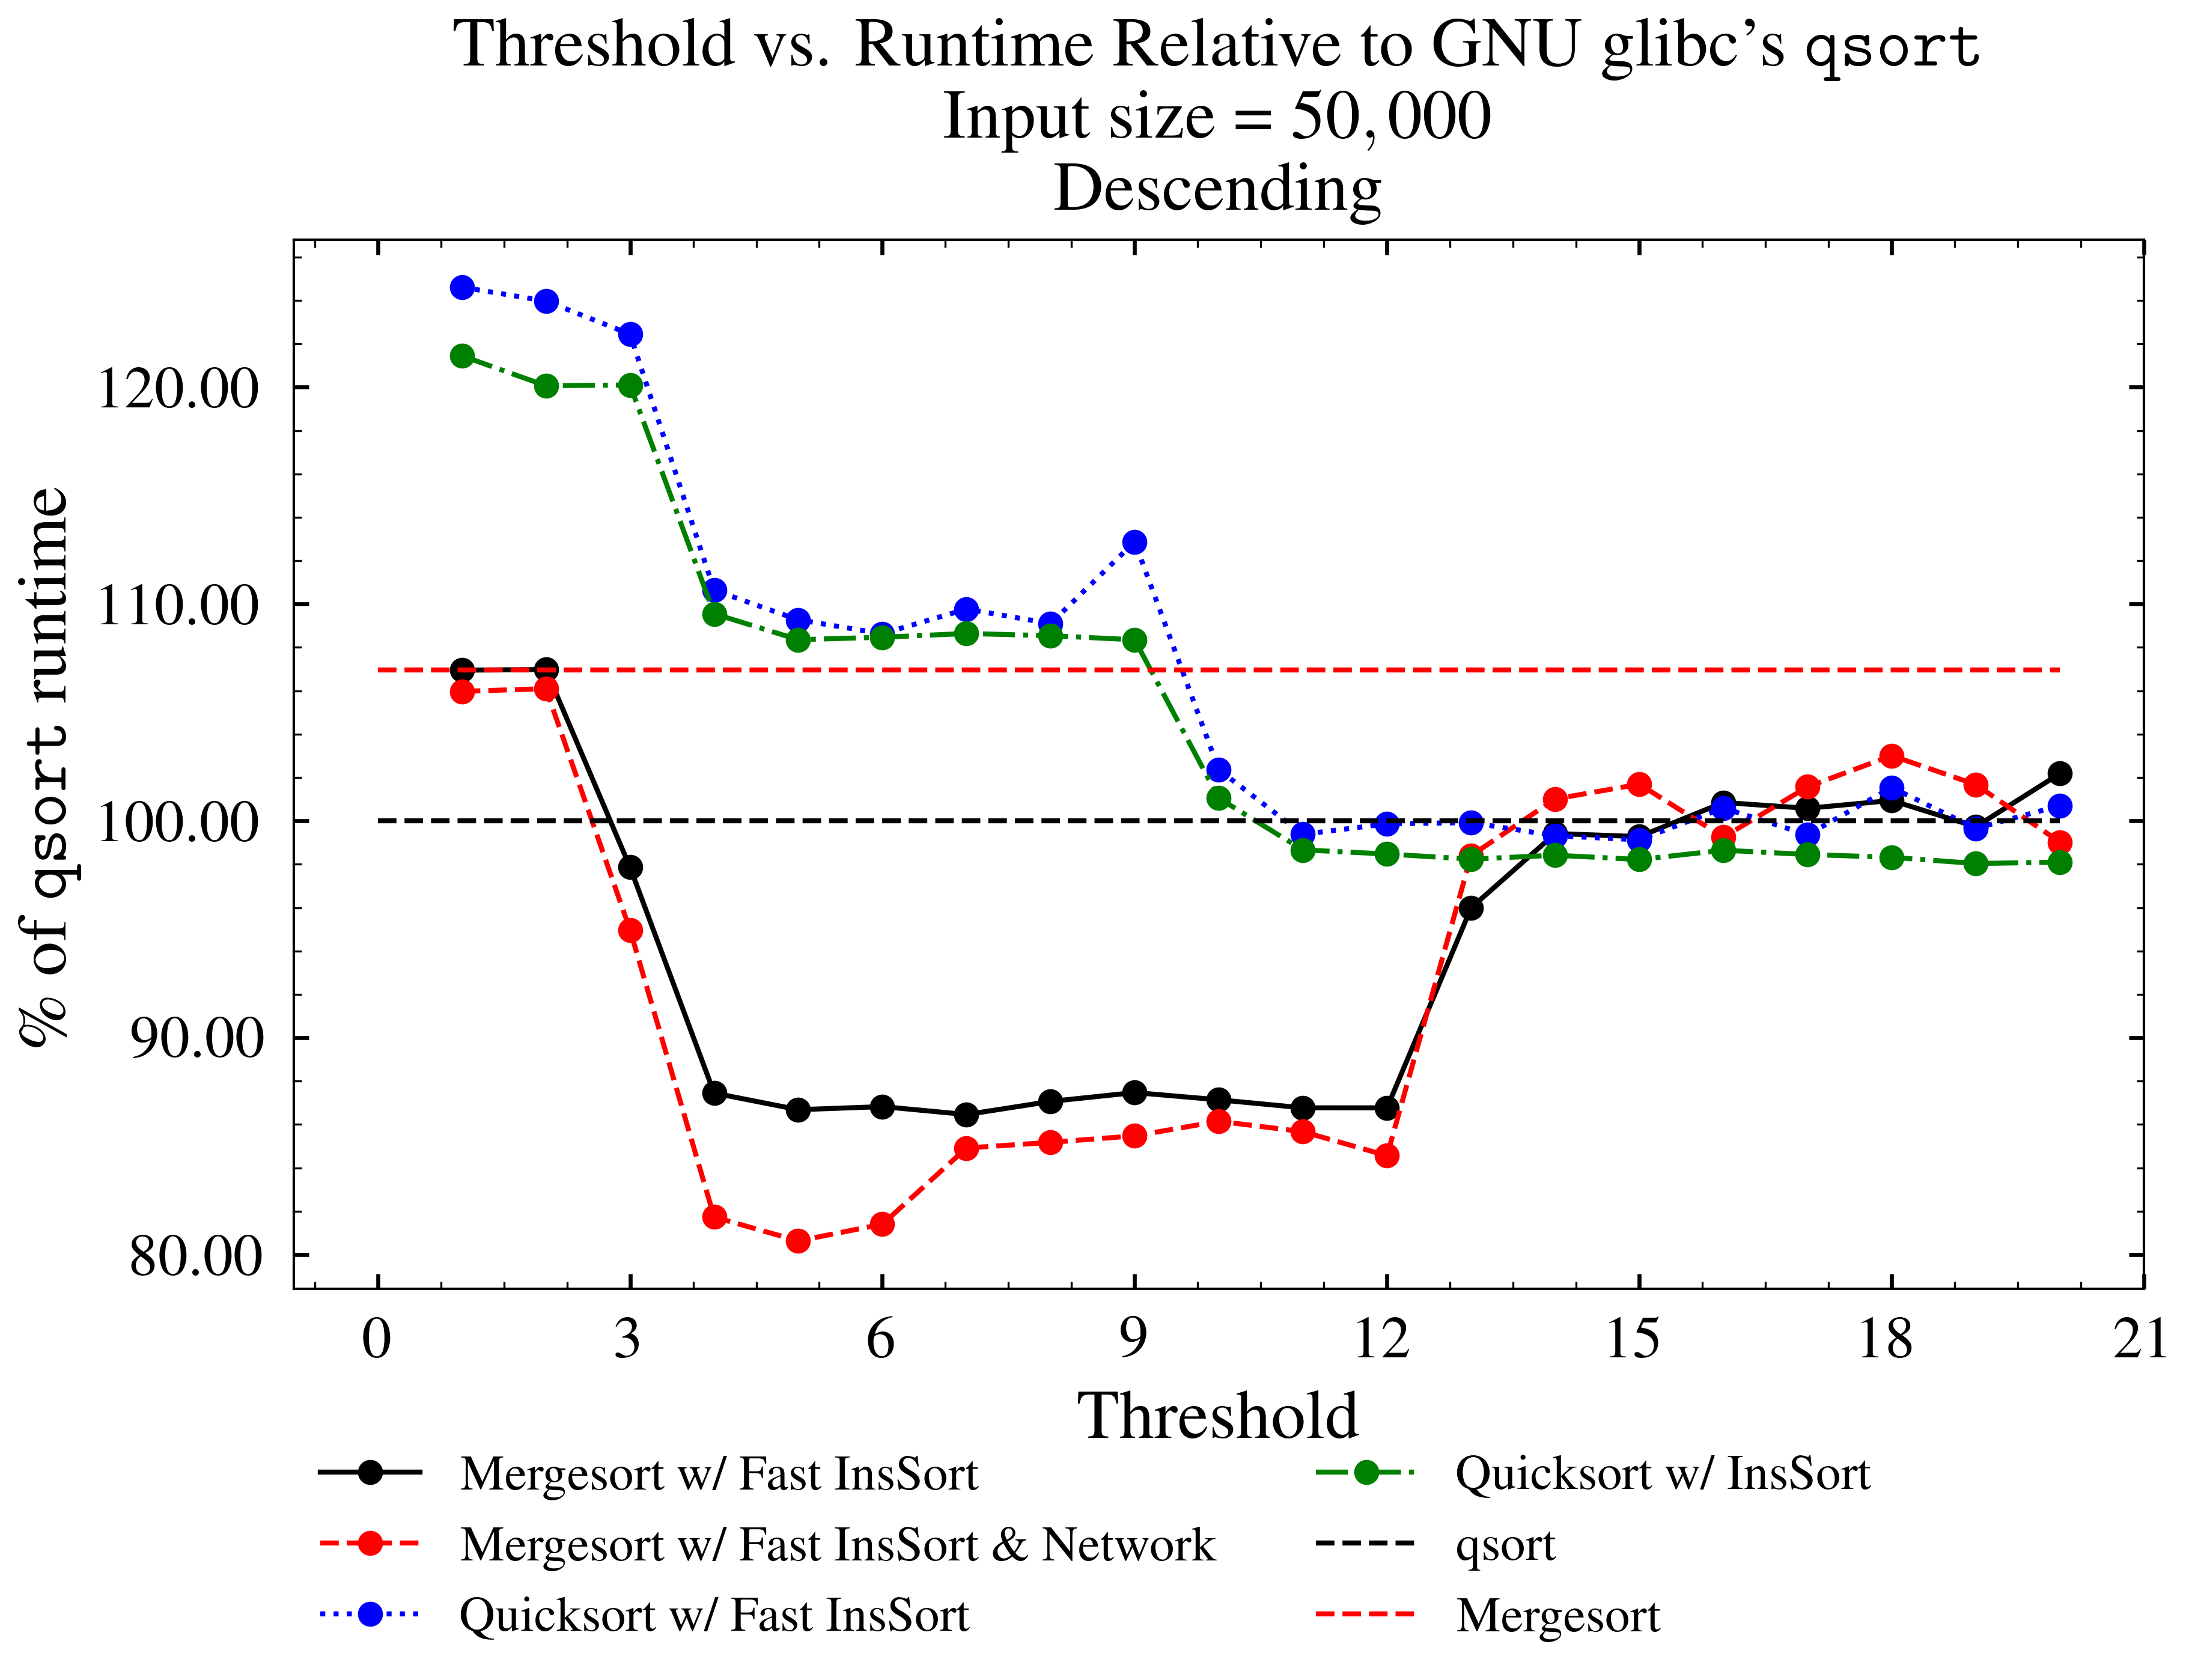
\includegraphics[width=\columnwidth]{descending}}
	\caption{Descending}
	\label{fig:descending}
\end{figure}
\begin{figure}[H]
	\centering
	\makebox[\columnwidth]{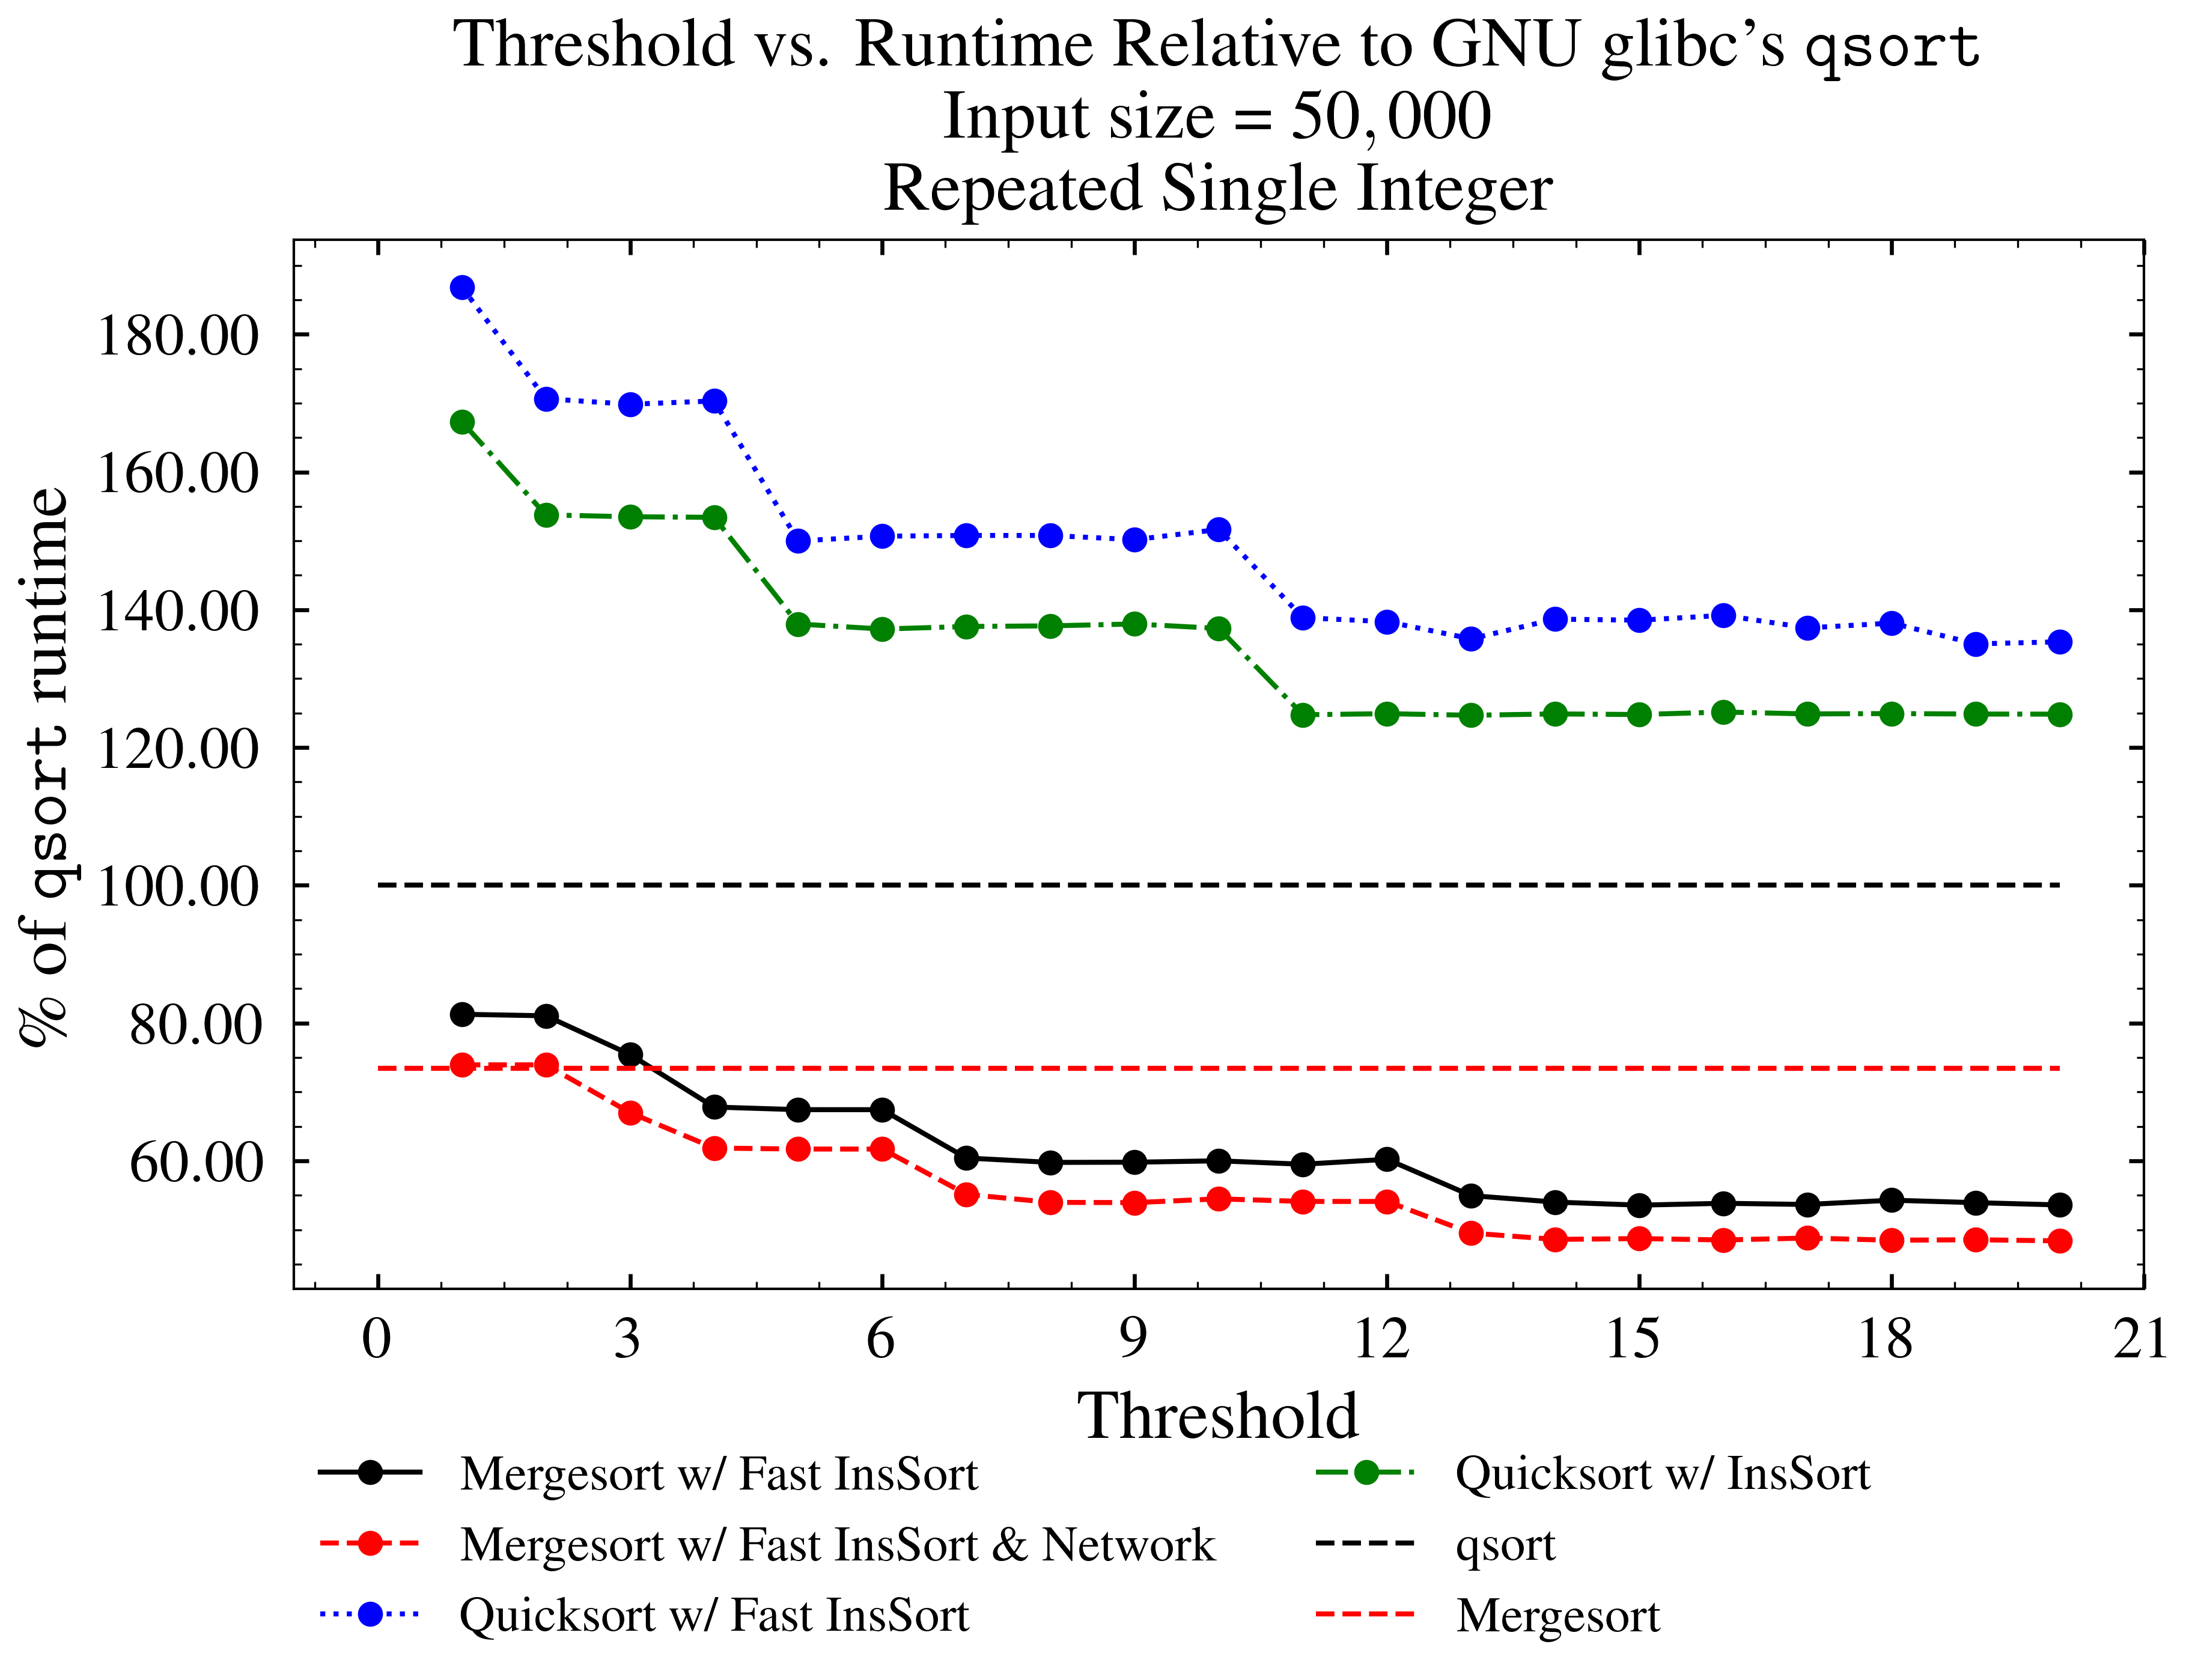
\includegraphics[width=\columnwidth]{single_num}}
	\caption{Single Num}
	\label{fig:single_num}
\end{figure}

\section{CONCLUSION}

\todo

%%%%%%%%%%%%%%%%%%%%%%%%%%%%%%%%%%%%%%%%%%%%%%%%%%%%%%%%%%%%%%%%%%%%%%%%%%%%%%%%

% This command serves to balance the column lengths on the last page of the
% document manually. It shortens the textheight of the last page by a suitable
% amount. This command does not take effect until the next page so it should
% come on the page before the last. Make sure that you do not shorten the
% textheight too much.
% \addtolength{\textheight}{-12cm}

% \titleformat*{\section}{\fontsize{12pt}{14pt}\MakeUppercase\selectfont}
\printbibliography
\end{document}
